\documentclass[10pt]{beamer}

\usetheme{Frankfurt}

%%% Работа с русским языком
\usepackage{cmap}					% поиск в PDF
\usepackage{mathtext} 				% русские буквы в формулах
\usepackage[T2A]{fontenc}			% кодировка
\usepackage[utf8]{inputenc}			% кодировка исходного текста
\usepackage[english,russian]{babel}	% локализация и переносы
\usepackage{indentfirst}
\frenchspacing


%%% Дополнительная работа с математикой
\usepackage{amsmath,amsfonts,amssymb,amsthm,mathtools} % AMS
\usepackage{icomma} % "Умная" запятая: $0,2$ --- число, $0, 2$ --- перечисление

%% Номера формул
%\mathtoolsset{showonlyrefs=true} % Показывать номера только у тех формул, на которые есть \eqref{} в тексте.
%\usepackage{leqno} % Нумерация формул слева

%% Свои команды
\DeclareMathOperator{\sgn}{\mathop{sgn}}

%% Перенос знаков в формулах (по Львовскому)
\newcommand*{\hm}[1]{#1\nobreak\discretionary{}
	{\hbox{$\mathsurround=0pt #1$}}{}}

%%% Работа с картинками
\usepackage{graphicx}  % Для вставки рисунков
\graphicspath{{images/}}  % папки с картинками
\setlength\fboxsep{3pt} % Отступ рамки \fbox{} от рисунка
\setlength\fboxrule{1pt} % Толщина линий рамки \fbox{}
\usepackage{wrapfig} % Обтекание рисунков текстом
\usepackage{subfigure}

%%% Работа с таблицами
\usepackage{array,tabularx,tabulary,booktabs} % Дополнительная работа с таблицами
\usepackage{longtable}  % Длинные таблицы
\usepackage{multirow} % Слияние строк в таблице

%%% Программирование
\usepackage{etoolbox} % логические операторы

%
%\usepackage{fancyhdr} % Колонтитулы
% 	\pagestyle{fancy}
%\renewcommand{\headrulewidth}{0pt}  % Толщина линейки, отчеркивающей верхний колонтитул
% 	\lfoot{Нижний левый}
% 	\rfoot{Нижний правый}
% 	\rhead{Верхний правый}
% 	\chead{Верхний в центре}
% 	\lhead{Верхний левый}
%	\cfoot{Нижний в центре} % По умолчанию здесь номер страницы

\usepackage{setspace} % Интерлиньяж
%\onehalfspacing % Интерлиньяж 1.5
%\doublespacing % Интерлиньяж 2
%\singlespacing % Интерлиньяж 1

\usepackage{lastpage} % Узнать, сколько всего страниц в документе.

\usepackage{soul} % Модификаторы начертания


\usepackage{csquotes} % Еще инструменты для ссылок

%\usepackage[style=authoryear,maxcitenames=2,backend=biber,sorting=nty]{biblatex}

\usepackage{multicol} % Несколько колонок

\usepackage{tikz} % Работа с графикой
\usepackage{pgfplots}
\usepackage{pgfplotstable}

\renewcommand{\phi}{\varphi}
\renewcommand{\epsilon}{\varepsilon}
\usepackage[justification=centering, font=footnotesize]{caption}
\setbeamertemplate{caption}[numbered]

\newcommand{\delayV}[1]{\overset{\leftarrow}{\textbf{x}}_{#1}}
\newcommand{\delayM}[1]{\overset{\leftarrow}{\mathbf{X}}_{#1}}

\theoremstyle{definition}
\newtheorem*{Def}{Определение}

\usepackage{grffile}
%\usepackage{graphicx}

\setlength{\parskip}{0.1cm}

\date{2024}
\title{Тензорная декомпозиция и прогноз для набора временных рядов}
\author{Сёмкин Кирилл \inst{1}  \and Вадим Стрижов \inst{2}}
\institute{\inst{1}  Московский физико-технический институт \and \inst{2} д.ф.-м.н., Московский физико-технический институт}

\begin{document}
	
	\begin{frame}[c]
		\titlepage
	\end{frame}

	\begin{frame}{Мотивация}
		
		\begin{alertblock}{Проблема}
			Обработка многомерных временных рядов влечёт необходимость учёта взаимосвязей сигналов. Нейросетевые и статистические методы имеют большое количество параметров, и требуют изощрённых процедур обучения. При этом они не предлагают способа построения декомпозиции.
		\end{alertblock}
		
		\begin{figure}[h]
			\centering
			
			\includegraphics[width=0.69\textheight, keepaspectratio]{img/prey_predetor_graph}
			\includegraphics[width=0.28\textheight, keepaspectratio]{img/hare-lynx.jpg}
			
			\caption{График количества особей хищников и жертв от времени}
			
		\end{figure}
		
	\end{frame}
	
	\begin{frame}{Цель исследования}
		
		Предложить метод, позволяющий выделить общую для набора сигналов структуру. На её основании произвести разложение каждого сигнала на компоненты. Найти способ построения прогноза.
		
		\begin{exampleblock}{Решение}
			\textbf{tSSA} = модель собственного пространства сигнала + тензорное представление данных + CPD
		\end{exampleblock}
		
		Подход опирается на гипотезу порождения динамической системой и является расширением метода SSA.
		
	\end{frame}
	
	\begin{frame}{Постановка задачи}
		
		\emph{Динамическая система} в дискретном времени:
		
		\begin{equation*}
			\begin{cases}
				\textbf{y}(t + 1) = f(\textbf{y}(t)), \ t \in \mathbb{N} \\
				\textbf{y}(0) = \textbf{y}_0
			\end{cases}
		\end{equation*}
		
		$ \textbf{y} \in X $, где $ X $ --- гладкое многообразие большой размерности. 
		
		Конкретная траектория этой системы \emph{порождает} наблюдаемые ряды через некое многомерное отображение $ \boldsymbol{\phi}: X \to \mathbb{R}^m $:
		
		\begin{equation*}
			\boldsymbol{\phi}(\textbf{y}(t)) = \textbf{x}_t \Leftrightarrow \begin{cases}
				\phi_1(\textbf{y}(t)) = x_1(t) \\
				\ldots \\
				\phi_m(\textbf{y}(t)) = x_m(t) \\
			\end{cases}
		\end{equation*}
		
	\end{frame}
	
	\begin{frame}{Постановка задачи}
		
		Выдвигается гипотеза, что траектории $ \textbf{y}(t) $ лежат в многообразии $ M \subset X $ размерности  меньшей, чем у $ X $. Ставится задача поиска вложения (embedding) $ M $ в $ \mathbb{R}^{L} $ для некоторого $ L $ и нахождения базиса в образе этого вложения.
		
		\begin{figure}[h]
			\centering
			
			\includegraphics[width=0.6\textheight, keepaspectratio]{img/dynamic_system_example.png}
			\caption{Динамическая система собственной размерности < 3}
			
		\end{figure}
		
	\end{frame}
	
	\begin{frame}{Поиск решения}
		
		\begin{theorem}[Такенс]
			Искомое вложение даётся построением соответствующего вектора задержки 
			
			\begin{equation*}
				\textbf{y}(t) \xrightarrow{emb} \begin{pmatrix}
					\boldsymbol{\phi} \circ f^{t - L + 1}(\textbf{y}(t)) \\
					\vdots \\
					\boldsymbol{\phi} \circ f(\textbf{y}(t)) \\
					\boldsymbol{\phi} \circ \textbf{y}(t)
				\end{pmatrix} = \begin{pmatrix}
					x(t - L + 1) \\
					\vdots \\
					x(t - 1) \\
					x(t)
				\end{pmatrix} = \delayV{t} \in \mathbb{R}^L
			\end{equation*}
			
		\end{theorem}
		
		Полученное пространство вложения $ \text{Lin}(\{\delayV{t}\}) $ и есть \emph{собственное пространство сигнала} $ x(t) $.
		
		C помощью разложения \emph{траекторной матрицы} $ \mathbf{H}_x = [ \delayV{1} \ldots  \delayV{N - L + 1}]. $ выделяем в нём базис. Далее можем декомпозировать и строить прогноз (SSA). 
	
	\end{frame}
	
	\begin{frame}{Метод tSSA}
		
		В случае нескольких рядов упакуем их вектора задержек в \emph{матрицы задержек} $ ( \delayV{1_t} \ldots \delayV{m_t} ) := \delayM{t} $. Состыкуем их в \emph{траекторный тензор} $ \textbf{T} $.
		
		\begin{figure}[h]
			\centering
			\subfigure{\includegraphics[width=0.4\textwidth, keepaspectratio]{img/Trajectory_Tensor_1}}
			\subfigure{\includegraphics[width=0.4\textwidth, keepaspectratio]{img/Trajectory_Tensor_2}}
			
			\caption{Два вида на $ \textbf{T} $. Слева --- в виде набора траекторных матриц сигналов. Справа --- в виде набора матриц задержки.}\label{pic:traj_tensor}
		\end{figure}
		
	\end{frame}
	
	\begin{frame}{Метод tSSA}
		
		Применим \textit{CPD-разложение} к траекторному тензору и рассмотрим его вид для каждого сечения по третьему измерению:
		
		\begin{equation*}\label{eq:tSSA_decomp}
			\textbf{T} = \sum\limits_{i = 1}^{r} \mathbf{a}_i \otimes \mathbf{b}_i \otimes \mathbf{c}_i \Leftrightarrow \begin{cases}
				\mathbf{H}_{x_1} = \sum\limits^{r} \boldsymbol{\sigma}_{x_1}(i) \cdot \mathbf{a}_i  \mathbf{b}_i^{\mathsf{T}}  \\
				\mathbf{H}_{x_2} = \sum\limits^{r} \boldsymbol{\sigma}_{x_2}(i) \cdot \mathbf{a}_i  \mathbf{b}_i^{\mathsf{T}} \\
				\ldots \\
				\mathbf{H}_{x_m} = \sum\limits^{r} \boldsymbol{\sigma}_{x_m}(i) \cdot \mathbf{a}_i  \mathbf{b}_i^{\mathsf{T}} 
			\end{cases}
		\end{equation*}
		
		Получили разложение траекторных матриц сигналов по \emph{общему базису}, что и выражает взаимосвязанность рядов.
		
	\end{frame}
	
	\begin{frame}{Декомпозиция сигналов}
		
		Для получения декомпозиции факторы разложения $ \mathbf{H}_{x_k} $ разбиваем на группы и \emph{ганкелизуем} --- усредняем матрицы по антидиагоналям.
		
		\begin{multline*}
			\mathbf{H}_{x_k} = \sum\limits_{i = 1}^{r} \boldsymbol{\sigma}_{x_k}(i) \cdot \mathbf{a}_i  \mathbf{b}_i^{\mathsf{T}} = \sum\limits_{i \in \mathbb{I}_1} \boldsymbol{\sigma}_{x_k}(i) \cdot \mathbf{a}_i  \mathbf{b}_i^{\mathsf{T}} + \ldots + \sum\limits_{i \in \mathbb{I}_s} \boldsymbol{\sigma}_{x_k}(i) \cdot \mathbf{a}_i  \mathbf{b}_i^{\mathsf{T}} = \\ = C_1 + \ldots + C_s = \text{Hankel}(C_1) + \ldots + \text{Hankel}(C_s)  \Leftrightarrow x_k(t) = c_1(t) + \ldots c_s(t)
		\end{multline*}
		
		\begin{alertblock}{Проблема}
			Хочется группировать факторы так, что каждая матрица $ C_i $ была как можно более "<ганкелевой">. Это бы усилило связь разложения траекторной матрицы и самого сигнала.
		\end{alertblock}
		
	\end{frame}
	
	\begin{frame}{Оптимальная декомпозиция}
		
		\only<1>{
			Обозначим невязку $ H_i = \boldsymbol{\sigma}_{x_k}(i) \cdot \mathbf{a}_i  \mathbf{b}_i^{\mathsf{T}} - Hankel(\boldsymbol{\sigma}_{x_k}(i) \cdot \mathbf{a}_i  \mathbf{b}_i^{\mathsf{T}}) $, тогда из предыдущего выражения следует:
			
			\begin{equation*}
				H_1 + \ldots + H_r = 0 \Leftrightarrow H_r = - \sum\limits_{j = 1}^{r - 1} H_j
			\end{equation*}
			
			Раскладываем на две группы. В каждой хотя бы две невязки, вместе суммирующиеся в ноль. Т.о. условие оптимальной декомпозиции:
			
			\begin{equation*}
				\begin{cases*}
					\sum\limits_{j = 1}^{r - 1} \beta_j H_j = 0 \\
					\beta_j \in \{0, 1\}, \ \forall j \in 1, \ldots, r \\
					\sum\limits_{i = 1}^{r - 1} \beta_j \ge 2
				\end{cases*} \Rightarrow
				\begin{cases*}
					\lVert \Lambda \boldsymbol{\beta} \rVert \to \underset{\boldsymbol{\beta}}{\min} \\
					\beta_j \in \{0, 1\}, \ \forall j \in 1, \ldots, r \\
					\sum\limits_{i = 1}^{r - 1} \beta_j \ge 2
				\end{cases*}
			\end{equation*}
		}
		
		\only<2>{
			Раскладываем на две группы. В каждой хотя бы две невязки, вместе суммирующиеся в ноль. Т.о. условие оптимальной декомпозиции:
			
			\begin{equation*}
				\begin{cases*}
					\lVert \Lambda \boldsymbol{\beta} \rVert \to \underset{\boldsymbol{\beta}}{\min} \\
					\beta_j \in \{0, 1\}, \ \forall j \in 1, \ldots, r \\
					\sum\limits_{i = 1}^{r - 1} \beta_j \ge 2
				\end{cases*}
			\end{equation*}
			
			Имеем задачу наименьших квадратов с целочисленными ограничениями (ILS), которая является NP-сложной.
		}
		
	\end{frame}
	
	\begin{frame}{Прогнозирование}
		
		Базис в пространстве векторов задержек сигнала даётся как $ \text{Lin}(\{\mathbf{a}_i\}) \Leftrightarrow A = [\mathbf{a}_1 \ldots \mathbf{a}_r] $. 
		
		Прогноз на один шаг вперёд сводится к решению частично неизвестной СЛАУ:
		
		\begin{gather*}\label{eq:main_pred_for_A}
			\delayV{N + 1} = A \boldsymbol{\lambda} \Leftrightarrow \begin{cases}
				\mathbf{x}_{kn} = A_{kn} \boldsymbol{\lambda}  \\
				x(N + 1) = \mathbf{a}_{pr}^{\mathsf{T}} \boldsymbol{\lambda}
			\end{cases}, \text{ где } \\
			A = \left( \dfrac{A_{kn}}{\mathbf{a}_{pr}^{\mathsf{T}}} \right) \nonumber \\
			\delayV{N + 1} = (\mathbf{x}_{kn}, \  x(N + 1))^{\mathsf{T}} \nonumber
		\end{gather*}
		
		Из-за переопределённости системы, решение выражается в смысле наименьших квадратов:
		
		\begin{equation*}
			x(N + 1) = \mathbf{a}_{pr}^{\mathsf{T}} (A_{kn}^T A_{kn})^{-1} A_{kn}^T \mathbf{x}_{kn}
		\end{equation*}
		
		% TODO: сказать здесь о авторегрессии
		
	\end{frame}
	
	\begin{frame}{Вычислительный эксперимент}
		
		Цель: 
		
		\begin{itemize}
			\item применить метод tSSA для декомпозиции и прогноза многомерных временных рядов, а также сравнить его с другими моделями: mSSA, VAR, RNN
		\end{itemize}
		
		Рассматриваемые ряды:
		
		 \begin{itemize}
		 	\item план выработки электричества на день и цена его производства
		 	\item метеорологические данные (температура, осадки, атмосферное давление)
		 \end{itemize}
		 
		 Метрики:
		 
		 \begin{itemize}
		 	\item MSE, MAPE для прогнозирования
		 	\item AHE, RHE для декомпозиции
		 \end{itemize}
		
	\end{frame}
	
	\begin{frame}{Вычислительный эксперимент}
		
		\begin{Def}
			\emph{Абсолютной ошибкой ганкелизации} матрицы M назовём 
			
			\[
			\text{AHE} = \lVert M - \text{Hankel}(M) \rVert_2
			\] 
		\end{Def}
		
		\begin{Def}		
			
			\emph{Относительной ошибкой ганкелизации} матрицы M назовём 
			
			\[
			\text{RHE} = \frac{\text{AHE}}{\lVert M \rVert_2} 
			\] 		
			
		\end{Def}
		
		AHE можно представлять как суммарное стандартное отклонение антидиагоналей матрицы. RHE её более интерпретируемая модификация, которая и будет использоваться далее. 
		
		Данные метрики будут применяться к матрицам группировки факторов $ C_i $.
	
	\end{frame}
	
	\begin{frame}{Данные}
		\setlength{\parskip}{0.0001cm}
		
		\begin{figure}[h]
			\centering
			\includegraphics[width=0.43\textwidth, keepaspectratio]{../../figs/Electricity_Production}
			\includegraphics[width=0.43\textwidth, keepaspectratio]{../../figs/Electricity_Price}
			\caption{Потребление электричества и его цены за единицу мощности}\label{fig:electr_data}
		\end{figure}
		
		\begin{figure}[h]
			\centering
			\includegraphics[width=0.43\textwidth, keepaspectratio]{../../figs/Temperature.png}
			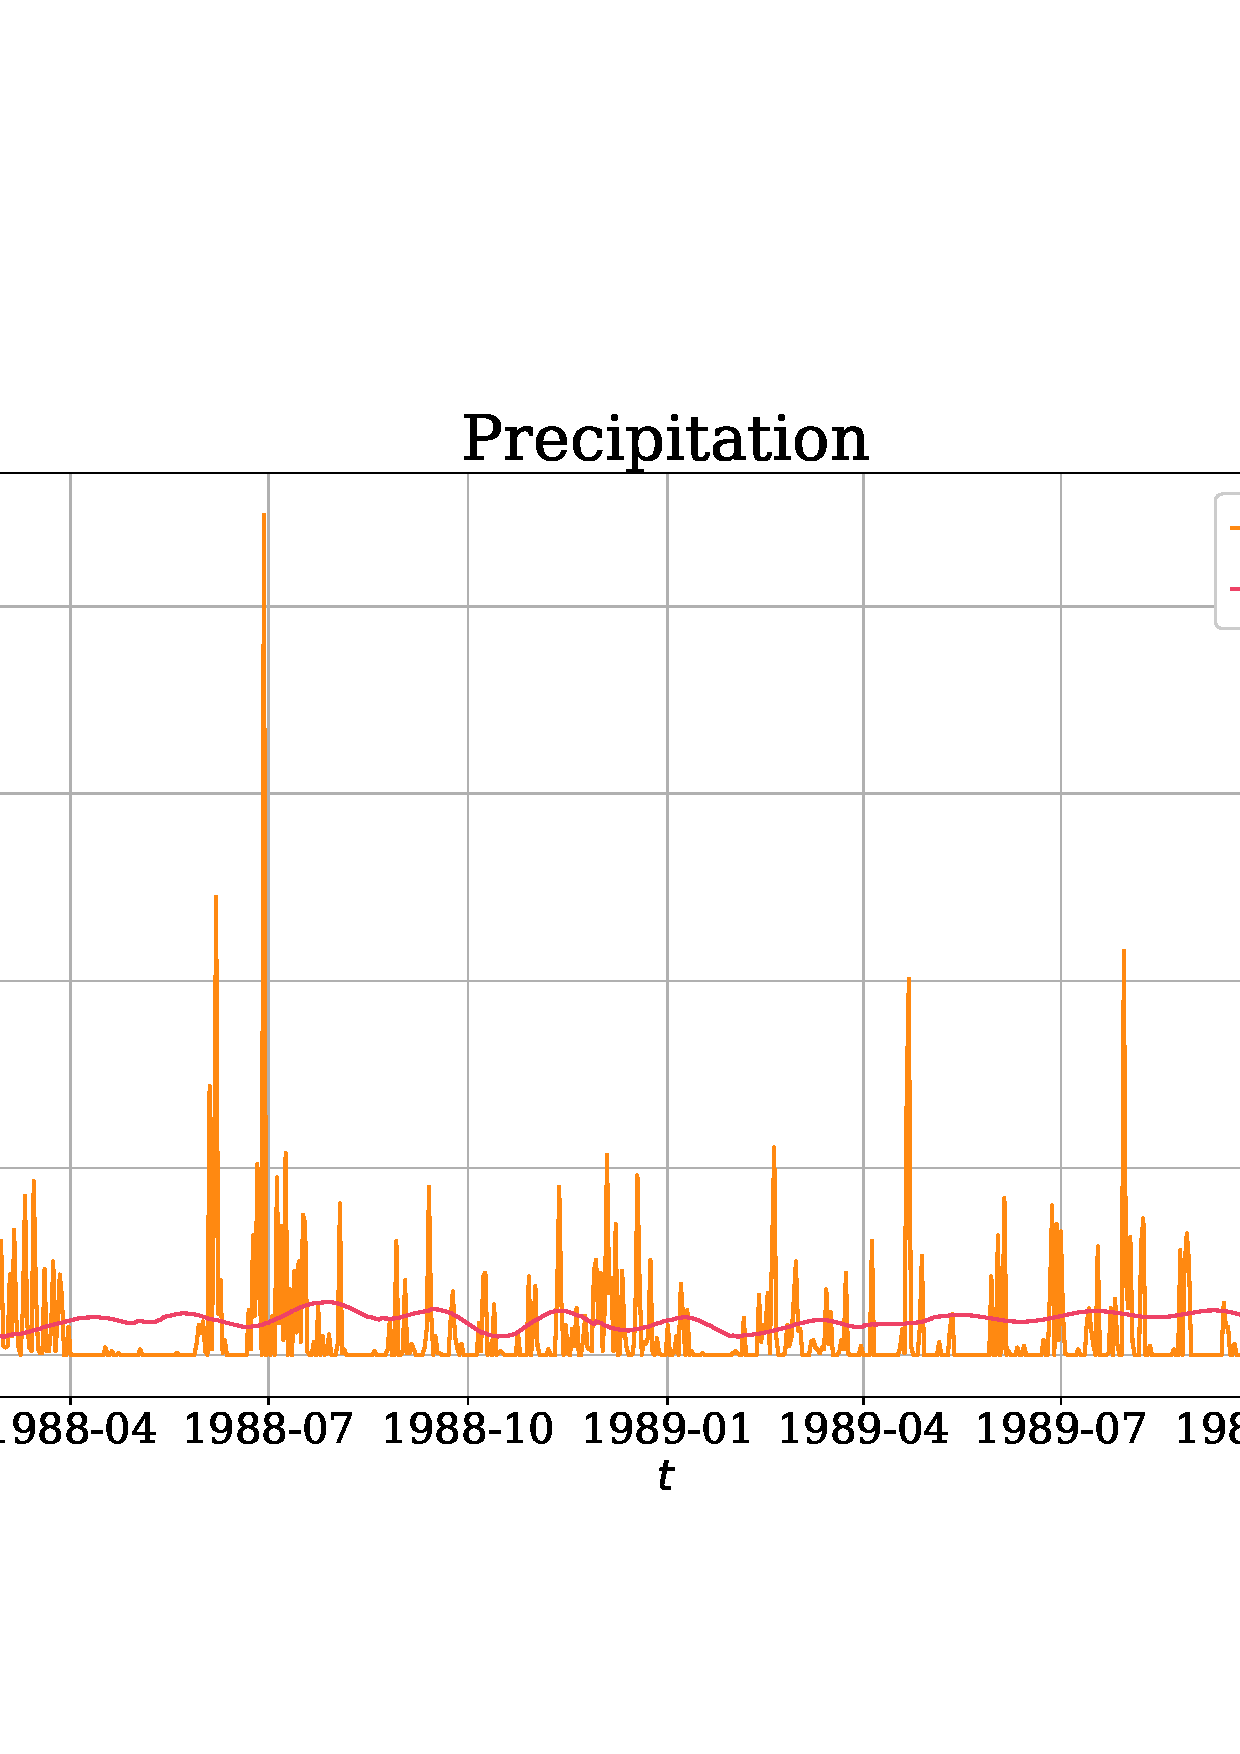
\includegraphics[width=0.43\textwidth, keepaspectratio]{../../figs/Precipitation.png}
			\includegraphics[width=0.43\textwidth, keepaspectratio]{../../figs/Pressure.png}
			\caption{Температура, осадки и давление, измеренные на метеостанции г. Берлин}\label{fig:weather_data}
		\end{figure}
		
	\end{frame}
	
	\begin{frame}{Электроэнергия. Прогноз}
		
		\only<1>{
			\begin{figure}[h]
				\centering
				\includegraphics[width=0.43\textwidth, keepaspectratio]{../../experiments/electricity/tssa/figs/prediction/MSE_rank.png}
				\includegraphics[width=0.43\textwidth, keepaspectratio]{../../experiments/electricity/tssa/figs/prediction/MAPE_rank.png}
				\caption{Значения метрик $ \overline{\text{MSE}} $ и $ \overline{\text{MAPE}} $ предсказания tSSA для разных рангов CP-разложения. Отдельно выделен оптимальный ранг.}\label{fig:mse_mape_electr}
			\end{figure}
				
				Наблюдается эффект переобучения при повышении значения ранга.
				
				\begin{figure}[h]
					\centering
					\includegraphics[width=0.43\textwidth, keepaspectratio]{../../experiments/electricity/tssa/figs/prediction/cpd_rank_30/Production_program.png}
					\includegraphics[width=0.43\textwidth, keepaspectratio]{../../experiments/electricity/tssa/figs/prediction/cpd_rank_30/Price.png}
					\caption{Предсказание данных электроэнергии методом tSSA. CPD-ранг $ = 30 $.}\label{fig:tssa_electr_pred}
				\end{figure}
		}
			 
		\only<2>{
			\def\arraystretch{1.1}
			\begin{table}[h]
				\centering
				\caption{Метрики моделей на прогнозировании данных электроэнергии}\label{tab:pred_res_electr}
				\begin{tabular}{|c|c|c|c|c|}
					\hline
					& \textit{tSSA}  & \textit{mSSA} & \textit{VAR} & \textit{RNN} \\ \hline
					$ \overline{\text{MSE}}_{\text{Producution}} $, $10^6$ & 1.24           & 1.51          & 7.81         & 2.70         \\ \hline
					$ \overline{\text{MSE}}_{\text{Price}} $, $10^3$      & 0.88           & 1.03          & 4.85         & 30.0         \\ \hline
					$ \overline{\text{MSE}} $, $10^6$             & \textbf{0.62}  & 0.75          & 3.91         & 135.00       \\ \hline
					$ \overline{\text{MAPE}}_{\text{Producution}} $        & 0.054          & 0.060         & 0.137        & 0.999        \\ \hline
					$ \overline{\text{MAPE}}_{\text{Price}} $             & 0.164          & 0.170         & 0.360        & 1.004        \\ \hline
					$ \overline{\text{MAPE}} $                    & \textbf{0.109} & 0.115         & 0.249        & 1.002        \\ \hline
				\end{tabular}
			\end{table}
			
			Наш метод показал наилучшие результаты, хотя mSSA был близок по точности. Метод VAR оказался нестабилен на выбранном горизонте прогнозирования, а RNN обучался в константную функцию.
		}
			 
	\end{frame}
	
	\begin{frame}{Электроэнергия. Декомпозиция}
		
		\begin{figure}[h]
			\centering
			\includegraphics[width=0.43\textwidth, keepaspectratio]{../../experiments/electricity/tssa/figs/decomposition/RHE_mean.png}
			\caption{Зависимость метрики $ \overline{\text{RHE}} $ от ранга CP-разложения. Данные электроэнергии. Отдельно выделен оптимальный ранг.}
		\end{figure}
		
		Метод tSSA достигает наибольшей обобщающей способности на небольших канонических рангах траекторных тензоров рядов, что подтверждает гипотезу о низкой собственной размерности данных.
		
	\end{frame}
	
	\begin{frame}{Электроэнергия. Декомпозиция}
		
		\begin{figure}[h]
			\centering
			\includegraphics[width=0.48\textwidth, keepaspectratio]{../../experiments/electricity/tssa/figs/decomposition/cpd_rank_20/Production_program.png}
			\includegraphics[width=0.48\textwidth, keepaspectratio]{../../experiments/electricity/tssa/figs/decomposition/cpd_rank_20/Price.png}
			\caption{Разложение рядов на две компоненты методом tSSA. Данные электроэнергии. CPD-ранг $ = 20 $}
		\end{figure} 
		
		В силу вычислительной сложности задачи ILS, разложение на б$\acute{\text{о}}$льшее количество компонент не производится. 
		
		Из графиков видно, как сильно общий базис сигналов влияет на их декомпозицию: компоненты рядов получились почти идентичными, с точностью до смещения и масштаба. Метод выдели две гармоники разных амплитуд.
		
	\end{frame}
	
	\begin{frame}{Электроэнергия. Декомпозиция}
		
		\def\arraystretch{1.1}
		\begin{table}[h]
			\centering
			\caption{Метрики моделей на декомпозиции данных электроэнергии}
			\begin{tabular}{|c|c|c|}
				\hline
				& tSSA  & mSSA           \\ \hline
				$ \overline{\text{RHE}}_{\text{Producution}} $  & 0.507 & 0.308          \\ \hline
				$ \overline{\text{RHE}}_{\text{Price}} $      & 0.511 & 0.31           \\ \hline
				$ \overline{\text{RHE}} $             & 0.509 & \textbf{0.309} \\ \hline
			\end{tabular}
		\end{table}
		
		Метод tSSA немного проигрывает по точности разложения. Кроме того, для него пока отсутствуют эвристики поиска оптимальных группировок, в отличие от mSSA. 
		
		Т.о. для tSSA необходимо или открывать собственные эмпирические закономерности, или менять принцип построения декомпозиции.
		
	\end{frame}
	
	\begin{frame}{Выносится на защиту}
		
		Тензорный метод tSSA был разработан для прогноза и декомпозиции набора временных рядов, обработка которых требует учёта фактора взаимосвязанности. Его главное достоинство --- проста в использовании: имеется всего два настраиваемых параметра, для которых не требуется изощрённых процедур обучения. Вместе с тем, теоретическое обоснование на основе довольно общей теории динамических систем. Главным вызовом метода является результат о NP-сложности поиска оптимальной декомпозиции рядов.
		
	\end{frame}
	
	\begin{frame}{Литература}
		
		\begin{itemize}
			\item D. Stepanov и N. Golyandina. «SSA-based approaches to analysis and forecast of multidimensional
			time series». В: Proceedings of the 5th St.Petersburg Workshop on Simulation. 2005,	с. 293—298.
			\item Floris Takens. «Detecting Strange Attractors in Turbulence». В: Dynamical Systems and Turbulence, Warwick 1980. Под ред. David Rand и Lai-Sang Young. Т. 898. Lecture	Notes in Mathematics. Berlin: Springer, 1981. Гл. 21, с. 366—381.
			\item Tamara Kolda и Brett Bader. «Tensor Decompositions and Applications». В: SIAM Review 51 (авг. 2009), с. 455—500.
		\end{itemize}
			
	\end{frame}
	
	
\end{document}